\documentclass[pdflatex,sn-vancouver-num]{sn-jnl}% Math and Physical Sciences Numbered Reference Style


\usepackage{amsfonts}%
\usepackage{mathrsfs}%
\usepackage[title]{appendix}%
\usepackage{textcomp}%
\usepackage{manyfoot}%
\usepackage{booktabs}%
\usepackage{algorithm}%
\usepackage{algorithmicx}%
\usepackage{algpseudocode}%

\usepackage{xcolor}
%\usepackage{tcolorbox}     % Color boxes
\usepackage{amsmath}       % Basic mathematical typesetting
\usepackage{amssymb}       % Advanced math symbols
\usepackage{amsthm}        % Theorems typesetting
%\usepackage{array}         % Advanced table column formats
%\usepackage{enumitem}      % Itemize/enumrate
%\usepackage{fancyhdr}      % Custom header/footer styles
%\usepackage{fourier}       % Adobe Utopia font
\usepackage{graphicx}      % Enhanced images support
%\usepackage{ifluatex}      % LuaTeX-specific options
%\usepackage{kantlipsum}    % English kantian-style lipsum
%\usepackage{lipsum}        % Lorem ipsum
\usepackage{listings}      % Code listings
%\usepackage{longtable}     % Multi-page tables
\usepackage{multirow}      % Advanced table cells
%\usepackage{setspace}      % Set space between lines
%\usepackage{scrextend}     % Allows \addmargin environment
%\usepackage{tablefootnote} % Table footnotes
%\usepackage{tocloft}       % Custom ToC/LoF/LoT
%\usepackage{url}           % URL-sensitive line breaks
%\usepackage{xspace}        % Remove duplicated spaces
%\usepackage{tabularx}

\usepackage{todonotes}
\setuptodonotes{inline}



\begin{document}

    %%=============================================================%%
    %% TITLE
    %%=============================================================%%

\title[Metagenomic Identification using Neural Networks]{Accelerating Metagenomic Identification of DNA Sequences Using Artificial Neural Networks
  }

    %%=============================================================%%
    %% AUTHOR(S)
    %%=============================================================%%

\author*[1]{\fnm{Patryk Filip} \sur{Gryz}}\email{patryk.gryz.stud@pw.edu.pl}
\author*[1]{\fnm{Robert} \sur{Nowak}}\email{robert.nowak@pw.edu.pl}

    \affil*[1]{\orgdiv{Institute of Computer Science}, \orgname{Warsaw University of Technology}, \orgaddress{\street{Nowowiejska 15/19}, \city{Warsaw}, \postcode{00-665}, \country{Poland}}}

    %%=============================================================%%
    %% ABSTRACT
    %% =============================================================%%




    \abstract{The rapid increase in the availability of DNA sequence data necessitates efficient and scalable methods for metagenomic identification. Traditional tools like BLAST, although accurate, often require significant computational resources and time, limiting their applicability to large datasets. Recent advances in artificial neural networks (ANNs) demonstrate their potential to address this issue by offering faster and more accurate solutions.

    This study introduces a novel ANN-based approach for the efficient metagenomic identification of DNA sequences. The proposed method reduces the complexity of large datasets by leveraging contrastive learning within an ANN to select representative sequences. This approach enhances computational efficiency by focusing classification efforts on these representatives rather than on the entire dataset. Comparative experiments were conducted on a benchmark dataset, evaluating the proposed ANN method alongside classical techniques such as k-mer embeddings and the Needleman-Wunsch algorithm.
    
    Experimental results revealed that the ANN-based approach achieves the highest weighted average classification quality among all tested methods, outperforming both classical approaches. Additionally, the ANN method demonstrates competitive execution times, benefiting from parallelized computations enabled by GPU processing.
    
    In conclusion, the study highlights the potential of ANN-based methods to bridge the gap between precision and scalability in genetic taxonomy. Future research directions include enhancing the network’s flexibility for varying sequence lengths and exploring its application for dimensionality reduction in broader bioinformatics tasks.}

    %%=============================================================%%
    %% KEYWORDS
    %%=============================================================%%

    \keywords{DNA sequencing, metagenomic identification, artificial neural networks, contrastive learning, sequence clustering}

    \maketitle

    %%=============================================================%%
    %% SECTIONS
    %%=============================================================%%

    \section{Background}
    The use of information about genetic material found in the environment, combined with sequence databases, enables metagenomic identification -- the identification of organisms present in a given sample.
    With the development of next-generation sequencing methods\cite{Reinartz:2002}, sequencing costs have decreased significantly, and the number of DNA sequences being analyzed has increased\cite{Muir:2016}.
    The time required for metagenomic identification using traditional tools, such as BLAST, is unacceptable in many applications -- can span several hours, even for relatively small collections of analyzed sequences (for example 4096 sequences),
    due to huge size and explosive growth of sequencing databases \cite{10.1093/nar/gkr854}.
    This process require significant computational resources. It is necessary to create new methods to allow analyzing new samples of data in acceptable time using available resources.

    The primary objective of this study is to propose fast and high quality metagenomic identification method. We propose usage an artificial neural network to support the selection of representative genetic sequences.
    Instead of classifying entire environmental genetic sequences sample, the proposed approach focuses on identifying a subset of sequences that best represent the sample.
    These selected representatives are then used to identification, reducing computational complexity while maintaining accuracy.

    Historically, one of the first algorithms that enabled metagenomic identification was the Needleman-Wunsch algorithm \cite{Needleman:1970}, developed in 1970, which allowed for the comparison of genetic sequences.
    However, the first solution that enabled this task within a reasonable time frame was a tool created in 1983 by D. Lipman and W. Wilbur \cite{Wilbur:1983}.
    Their method was based on dividing sequences into $k$-tuples, a generalization of $k$-mers, and comparing them.
    An advancement of this approach was the BLAST algorithm, introduced in 1990 \cite{Altschul:1990}, which also relied on $k$-mers and allowed for the efficient search of similar sequences in sequence databases.

    The metagenomic ideitification became popular over the past 15 years, due to sequence database growth.
    A notable example of interesting tool is the development of the MetaPhlAn tool in 2012 \cite{Segata:2012}, which uses marker genes to compare the species composition of metagenomic samples.
    Another marker gene-based approach is mOTUs2 \cite{Milanese:2019}, which identifies and analyzes markers unique to specific microbial strains.

    A different technique was employed in Centrifuge \cite{Kim:2016}, developed in 2016,
    which utilizes sequence indexing based on the Burrows-Wheeler transform \cite{Burrows:1994} and the Ferragina-Manzini index \cite{Ferragina:2000} for efficient sequences retrieval.
    A more classical approach is used in Kraken \cite{Wood:2014}, introduced in 2014, which combines $k$-mers with an indexed sequence database.
    An unconventional method for metageonomic identification was proposed in 2022 with BERTax \cite{Mock:2022}, which applies a transformer model \cite{Transformers} to DNA sequence analysis,
    treating DNA as a specialized language and allowing for classification without the need for reference databases.
    Another machine learning-based solution is CGRclust \cite{Alipour:2024}, which clusters DNA sequences using a two-dimensional chaos game representation and integrates unsupervised contrastive learning with convolutional neural networks.

    Currently we can propose three types of methods developed for metagenomic identification: methods using alignment, methods based on $k$-mers and methods using marker genes.
    Alignment-based tools should yield the best results, but they require significant computational resources.
    Algorithms based on $k$-mers are very fast, but they do not take into account all the information about the structure of the input genetic sequences, which reduces their quality.
    Solutions using marker genes are characterized by good quality, but they allow analysis only for subsets of organisms for which marker genes are known.

    Although recent years have seen studies on metagenomic identification using machine learning methods, there is still
    a lack of research focusing on the application of artificial neural networks with contrastive learning for efficient sequence clustering.
    In many fields, artificial neural networks (ANN) have demonstrated the ability to outperform classical heuristic algorithms, offering faster and more accurate results.
    By leveraging the capabilities of ANN, this works aims to accelerate metagenomic identification process while maintaining at least the same level of quality as traditional methods.
    Such an approach could significantly accelerate the classification process using available tools.

    The rest of the paper is organized as follows. Section 2 defines the problem, presents the proposed approach, and provides detailed implementation details.
    Section 3 describes the experimental setup, including used datasets, the performance metrics for evaluation, and the results obtained from experiments with analysis.
    Finally, section 4 concludes the paper by summarizing the main findings, discuss on the limtiations of proposed approach and suggesting potential directions for future research.

    \section{Methods}

    \todo{opisać potok, jest tekst w pracy inżynierskiej;
      tutaj trzeba dac ogolny opis metody, moze rysunek, gdzie jest pokazane grupowanie, pytanie bazy danych itd}

    \todo{tutaj elementy systemu}


    \subsection{\todo{czy to nie jest wybor reprezentanta?} Proposed Approach}

    The proposed method involves reducing the dimensionality of input DNA sequences to a feature vector in the form of $\mathbb{R}^{64}$ using an artificial neural network.
    The neural network employs contrastive learning, which enables the learning of representations while preserving dissimilarity between sequences.
    The dissimilarity between sequence representations will be calculated using cosine dissimilarity, expressed by the formula in equation \eqref{Equation:CosineDissimilarity}.

            \begin{equation}
                dsim(A, B) = 1 - sim(A, B)
                \label{Equation:CosineDissimilarity}
            \end{equation}

            where:
            \begin{align*}
                sim(A, B) =& \cos{\theta} = \frac{A \cdot B}{\|A\| \|B\|} = \frac{
                    \sum^{n}_{i = 1}A_i B_i
                }{
                    \sqrt{
                        \sum^{n}_{i = 1}A_i^2
                    }
                    \cdot
                    \sqrt{
                        \sum^{n}_{i = 1}B_i^2
                    }
                } \\
                A, B -& \text{compared vectors,} \\
                \theta -& \text{angle between $A$ and $B$,} \\
                A_j, B_j -& \text{$j$-th element of the vector $A$ and $B$, respectively.}
            \end{align*}

            \subsubsection{Artificial Neural Network}
                \paragraph{Architecture}
                The ANN model consists of two parts. The first part comprises two convolutional blocks with batch normalization and is responsible for feature extraction from the sequence. The second part utilizes fully connected layers with dropout and the GELU activation function \cite{Hendrycks:2016} and is connected to the first part of the model via a flattening layer.

                The model output is the output of the final linear layer, which is a feature vector of dimension \( \mathbb{R}^{64} \).

                Schematically, the architecture is presented in Figure~\ref{Picture:NeuralModel}.

                \begin{figure}[!htb]
                    \begin{center}
                        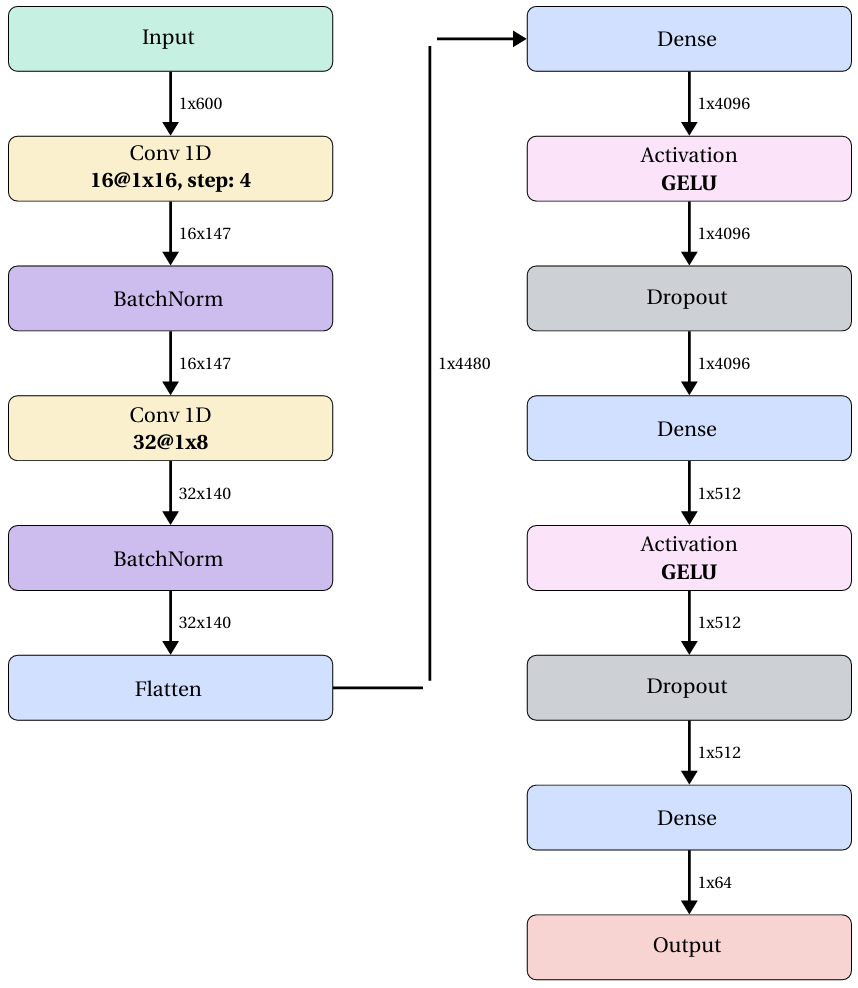
\includegraphics[width=\textwidth]{picture_ann_network.png}
                    \end{center}
                    \caption{
                        Diagram of ANN architecture.
                    }\label{Picture:NeuralModel}
                \end{figure}

                \paragraph{Input}
                The input to the model consists of DNA sequences of length $150$, which are encoded into a vector of dimensions $1 \times 600$ using one-hot encoding \cite{HarrisDavid:2007}.

                \paragraph{Training Examples}
                The training and validation examples consist of an anchor, a positive sequence that is similar to the anchor, and a negative sequence that is dissimilar to the anchor.

                \paragraph{Dataset}
                The training and validation datasets were created based on the first sample of genetic sequences from the CAMI II Toy Human Microbiome Project dataset \cite{Fritz:2019}. The sample contains simulated metagenomic data from the human skin microbiome. Examples were obtained by randomly selecting anchors from the dataset and modifying these anchors to create positive and negative sequences. The modification involved a point mutation of a given nucleotide to another one. In the case of positive sequences, the change affected between 0\% and 20\% of the anchor length, whereas for negative sequences, the change ranged from 20\% to 80\% of the anchor length.

                \paragraph{Loss function}
                The loss function used is defined as:

                \begin{equation}
                    \text{Contrastive loss} = [m_{pos} - s_{pos}]_{+} + [s_{neg} - m_{neg}]_{+}
                \end{equation}

                where:
                \begin{align*}
                    m_{pos} &- \text{similarity margin between the positive sequence and the anchor,} \\
                    m_{neg} &- \text{similarity margin between the negative sequence and the anchor,} \\
                    s_{pos} &- \text{cosine similarity of the positive sequence to the anchor,} \\
                    s_{pos} &- \text{cosine similarity of the negative sequence to the anchor.} \\
                \end{align*}
                
                \paragraph{Learning}
                The model was trained on a dataset of $10^{6}$ training examples and $10^{4}$ validation examples. The optimizer used was \textit{AdamW}\cite{Loshchilov2017DecoupledWD}.

                \paragraph{Quality}
                As a measure of model quality, the contrastive loss of the model was computed on the validation set.

                \paragraph{Parameters}
                Experiments were conducted to determine the optimal training parameters for the artificial neural network model. The tested parameters included the learning rate coefficient \( \lambda \), weight decay \( w \), the coefficient \( \gamma \) used in the exponential learning rate decay, the dropout rate, and the effectiveness of using three perceptron layers.

                As a result of these experiments, the best parameters were selected:
                \[
                \lambda = 10^{-6}, \quad w = , \quad \gamma = 0.99999
                \]
                a dropout rate of \( 0.5 \), and a confirmed positive impact of using three perceptron layers.

                Additionally, the loss function was used with the following parameters:
                \[
                m_{pos} = 1.0, \quad m_{neg} = 0.25.
                \]


                \paragraph{Results of Learning}
                As a result of training the neural network, the model achieved a validation set loss of $0.17$.

        % /\/\/\/\/\/\/\/\/\/\/\/\/\/\/\/\/\/\/\/\
        %   BEGIN REMOVED
        %       REASON: UNNECESSARY
        % /\/\/\/\/\/\/\/\/\/\/\/\/\/\/\/\/\/\/\/\

        \subsection{Implementation Details}
            The solution consists of two components. The first is a library that contains components enabling the creation of pipelines for genetic material analysis in the form of metagenomic identification. The second component is a console application, which uses the library's components to allow for the creation and configuration of processing pipelines. Additionally, a web application was created, which allows users to submit analysis tasks through a web browser.  

            The console application was implemented using the \textit{clap} library\cite{Rust:clap}. In library the $k$-medoid algorithm was provided by the \textit{kmedoids} library\cite{Rust:kmedoids}, and the neural network was built using the \textit{burn} library\cite{Rust:burn} with the \textit{wgpu} execution environment. Web application was implemented using the \textit{axum} library\cite{Rust:axum} with \textit{tokio}\cite{Rust:axum} async environment.

            Additionally, the following tools were used in the work:
            \begin{itemize}
                \item \textit{cargo} as the package manager and build system in Rust;
                \item \textit{rustup} for automatic management of Rust versions;
                \item \textit{clippy} for static code analysis in Rust;
                \item \textit{rustfmt} for automatic formatting of Rust source code;
                \item \textit{cargo test} for conducting unit tests;
                \item \textit{git} as the version control system, enabling change tracking and code history management.
            \end{itemize}

        % /\/\/\/\/\/\/\/\/\/\/\/\/\/\/\/\/\/\/\/\
        %   END REMOVED
        % /\/\/\/\/\/\/\/\/\/\/\/\/\/\/\/\/\/\/\/\

                \section{Results}

                This sections presents the results of the experiments conducted to evaluate the proposed solution, which aims to improve performance while maintaining the quality of metagenomic identifacation. The study involved comparing the new approach with two classical methods using the same dataset. The evaluation focused on execution time and identification quality to assess the effectiveness of the proposed approach.

        % /\/\/\/\/\/\/\/\/\/\/\/\/\/\/\/\/\/\/\/\
        %   BEGIN REMOVED
        %       REASON: UNNECESSARY
        % /\/\/\/\/\/\/\/\/\/\/\/\/\/\/\/\/\/\/\/\

        % \subsection{Experimental Setup}
        %     Experiments were conducted on the KVM based virtual machine with the specification given below:

        %     \begin{itemize}
        %         \item{
        %             \textbf{Operating System:} Ubuntu 22.04 LTS;
        %         }
        %         \item{
        %             \textbf{Processor:} 4 virtual cores of Intel Core i7-6850K;
        %         }
        %         \item{
        %             \textbf{RAM Memory:} 40 GB;
        %         }
        %         \item{
        %             \textbf{Graphics Card:} Nvidia GeForce GTX 1080 TI;
        %         }
        %         \item{
        %             \textbf{Disk:} 1 TB network drive with a read speed of 1 Gbps;
        %         }
        %         \item{
        %             \textbf{Software:} \texttt{BLAST} package version 2.16.0 and graphics card drivers.
        %         }
        %     \end{itemize}

        % /\/\/\/\/\/\/\/\/\/\/\/\/\/\/\/\/\/\/\/\
        %   END REMOVED
        % /\/\/\/\/\/\/\/\/\/\/\/\/\/\/\/\/\/\/\/\

        \subsection{Datasets}
            \subsubsection{Dataset Description}
                In the experiments, the \textit{CAMI II Toy Human Microbiome Project}\cite{Fritz:2019} dataset was used, which is the same dataset used for training the artificial neural network model. Dataset was chosen, because it was created for benchmarking bioinformatics tools and contains a large number of sequences, enabling its use both in experiments and in the learning process.

                Subsets of sequences were created from the dataset with sizes expressed by the formula $2^k$ for $k \in [0, 12]$. Subsets are disjoint, and only those sequences that were not used for training the ANN model were employed in their construction.

            \subsubsection{Dataset Preparation}
                The subsets were created by randomly sampling, without replacement, the indices of genetic sequences from the reference dataset that were to be included in each subset. Indices of sequences used in the training and validation sets of the ANN were excluded from the sampling. 


        \subsection{Base-line algorithms}

                \todo{tutaj metody klasyczne, porownawcze. PG: czy trzeba coś tutaj jeszcze dodawać?}

            Two classical approaches were implemented and used for comparison with the proposed neural network.

            \subsubsection{Modified Needleman-Wunsch Algorithm}
                The first classical approach is the Needleman-Wunsch algorithm. This algorithm allows for global alignment of genetic sequences. It uses a similarity matrix between sequences, which is constructed according to the rules given in equation~\eqref{Equation:NeedlemanWunsch}. A modification of the approach presented in equation~\eqref{Equation:NeedlemanWunschModified} is applied in the work.

                \begin{equation}
                    \begin{aligned}
                        D_{i,0} &= i \cdot g, & \text{for } & i \in [1, n + 1] \\
                        D_{0,j} &= j \cdot g, & \text{for } & j \in [2, m + 1] \\
                        D_{i,j} &= \max
                        \begin{cases}
                            D_{i - 1, j} + g \\
                            D_{i, j - 1} + g \\
                            D_{i - 1, j - 1} + s(A_i, B_j)
                        \end{cases}, & \text{for } & i \in (1, n + 1] \text{ and } j \in (1, m + 1]
                    \end{aligned}
                    \label{Equation:NeedlemanWunsch}
                \end{equation}

                where:
                \begin{align*}
                    A, B -& \text{compared sequences}, \\
                    n, m -& \text{lengths of sequences } A \text{ and } B, \\
                    D -& \text{similarity matrix of size } n + 1 \text{ x } m + 1, \\
                    g \in \mathbb{R} -& \text{penalty for a gap}, \\
                    s(A_i, B_j) \in \mathbb{R} -& \text{similarity between the } i\text{-th element in sequence A} \\ 
                                                & \text{ and the } j\text{-th element in sequence B}.
                \end{align*}

                \begin{equation}
                    \begin{aligned}
                        D_{i,j} &= \min
                        \begin{cases}
                        D_{i - 1, j} + g \\
                        D_{i, j - 1} + g \\
                        D_{i - 1, j - 1} + s(A_{i - 1}, B_{j - 1})
                        \end{cases}, & \text{for } & i \in \left(1, n + 1\right] \text{ and } j \in \left(1, m + 1\right] \\
                    \end{aligned}
                    \label{Equation:NeedlemanWunschModified}
                \end{equation}

                In the solution, the following parameter values were adopted:
                \begin{align*}
                    g &= 2, \\
                    s(a, b) &= \begin{cases}
                        0, & \text{for } a = b, \\
                        1, & \text{for } a \neq b.
                    \end{cases}
                \end{align*}

            \subsubsection{$k$-mer embeddings}
                The second approach will be the use of $k$-mers as embeddings, which allows for the representation of DNA sequences as numerical vectors. These vectors will then be compared using Euclidean distance.

        \subsection{Experiments}
            \subsubsection{Experiment 1: Metagenomic identification execution time}
                \paragraph{Objective} 
                Measuring the execution time of metagenomic identification using different genetic sequence clustering methods.

                \paragraph{Assumptions}
                \begin{enumerate}
                    \item {
                        Sequences clustering is deterministic.
                    }
                    \item {
                        Metagenomic identification is the only task running on the machine.
                    }
                \end{enumerate}

                \paragraph{Results}
                As a result of the experiment, the execution time for metagenomic identification was obtained for all methods. In the case of the method using the modified Needleman-Wunsch algorithm, results for metagenomic identification of 4096 sequences could not be obtained due to exceeding the execution time. Figure~\ref{Picture:Experiment:Duration} shows a graph of the metagenomic identification execution time as a function of the number of input sequences for: the method with the modified Needleman-Wunsch algorithm (NW), the method using $k$-mer embeddings ($k$-mer), the method using artificial neural networks (ANN), and for metagenomic identification of all sequences without using a pipeline (NP). Detailed execution times are provided in Table~\ref{Table:Experiment:Duration}.

                \begin{figure}[!htb]
                    \begin{center}
                        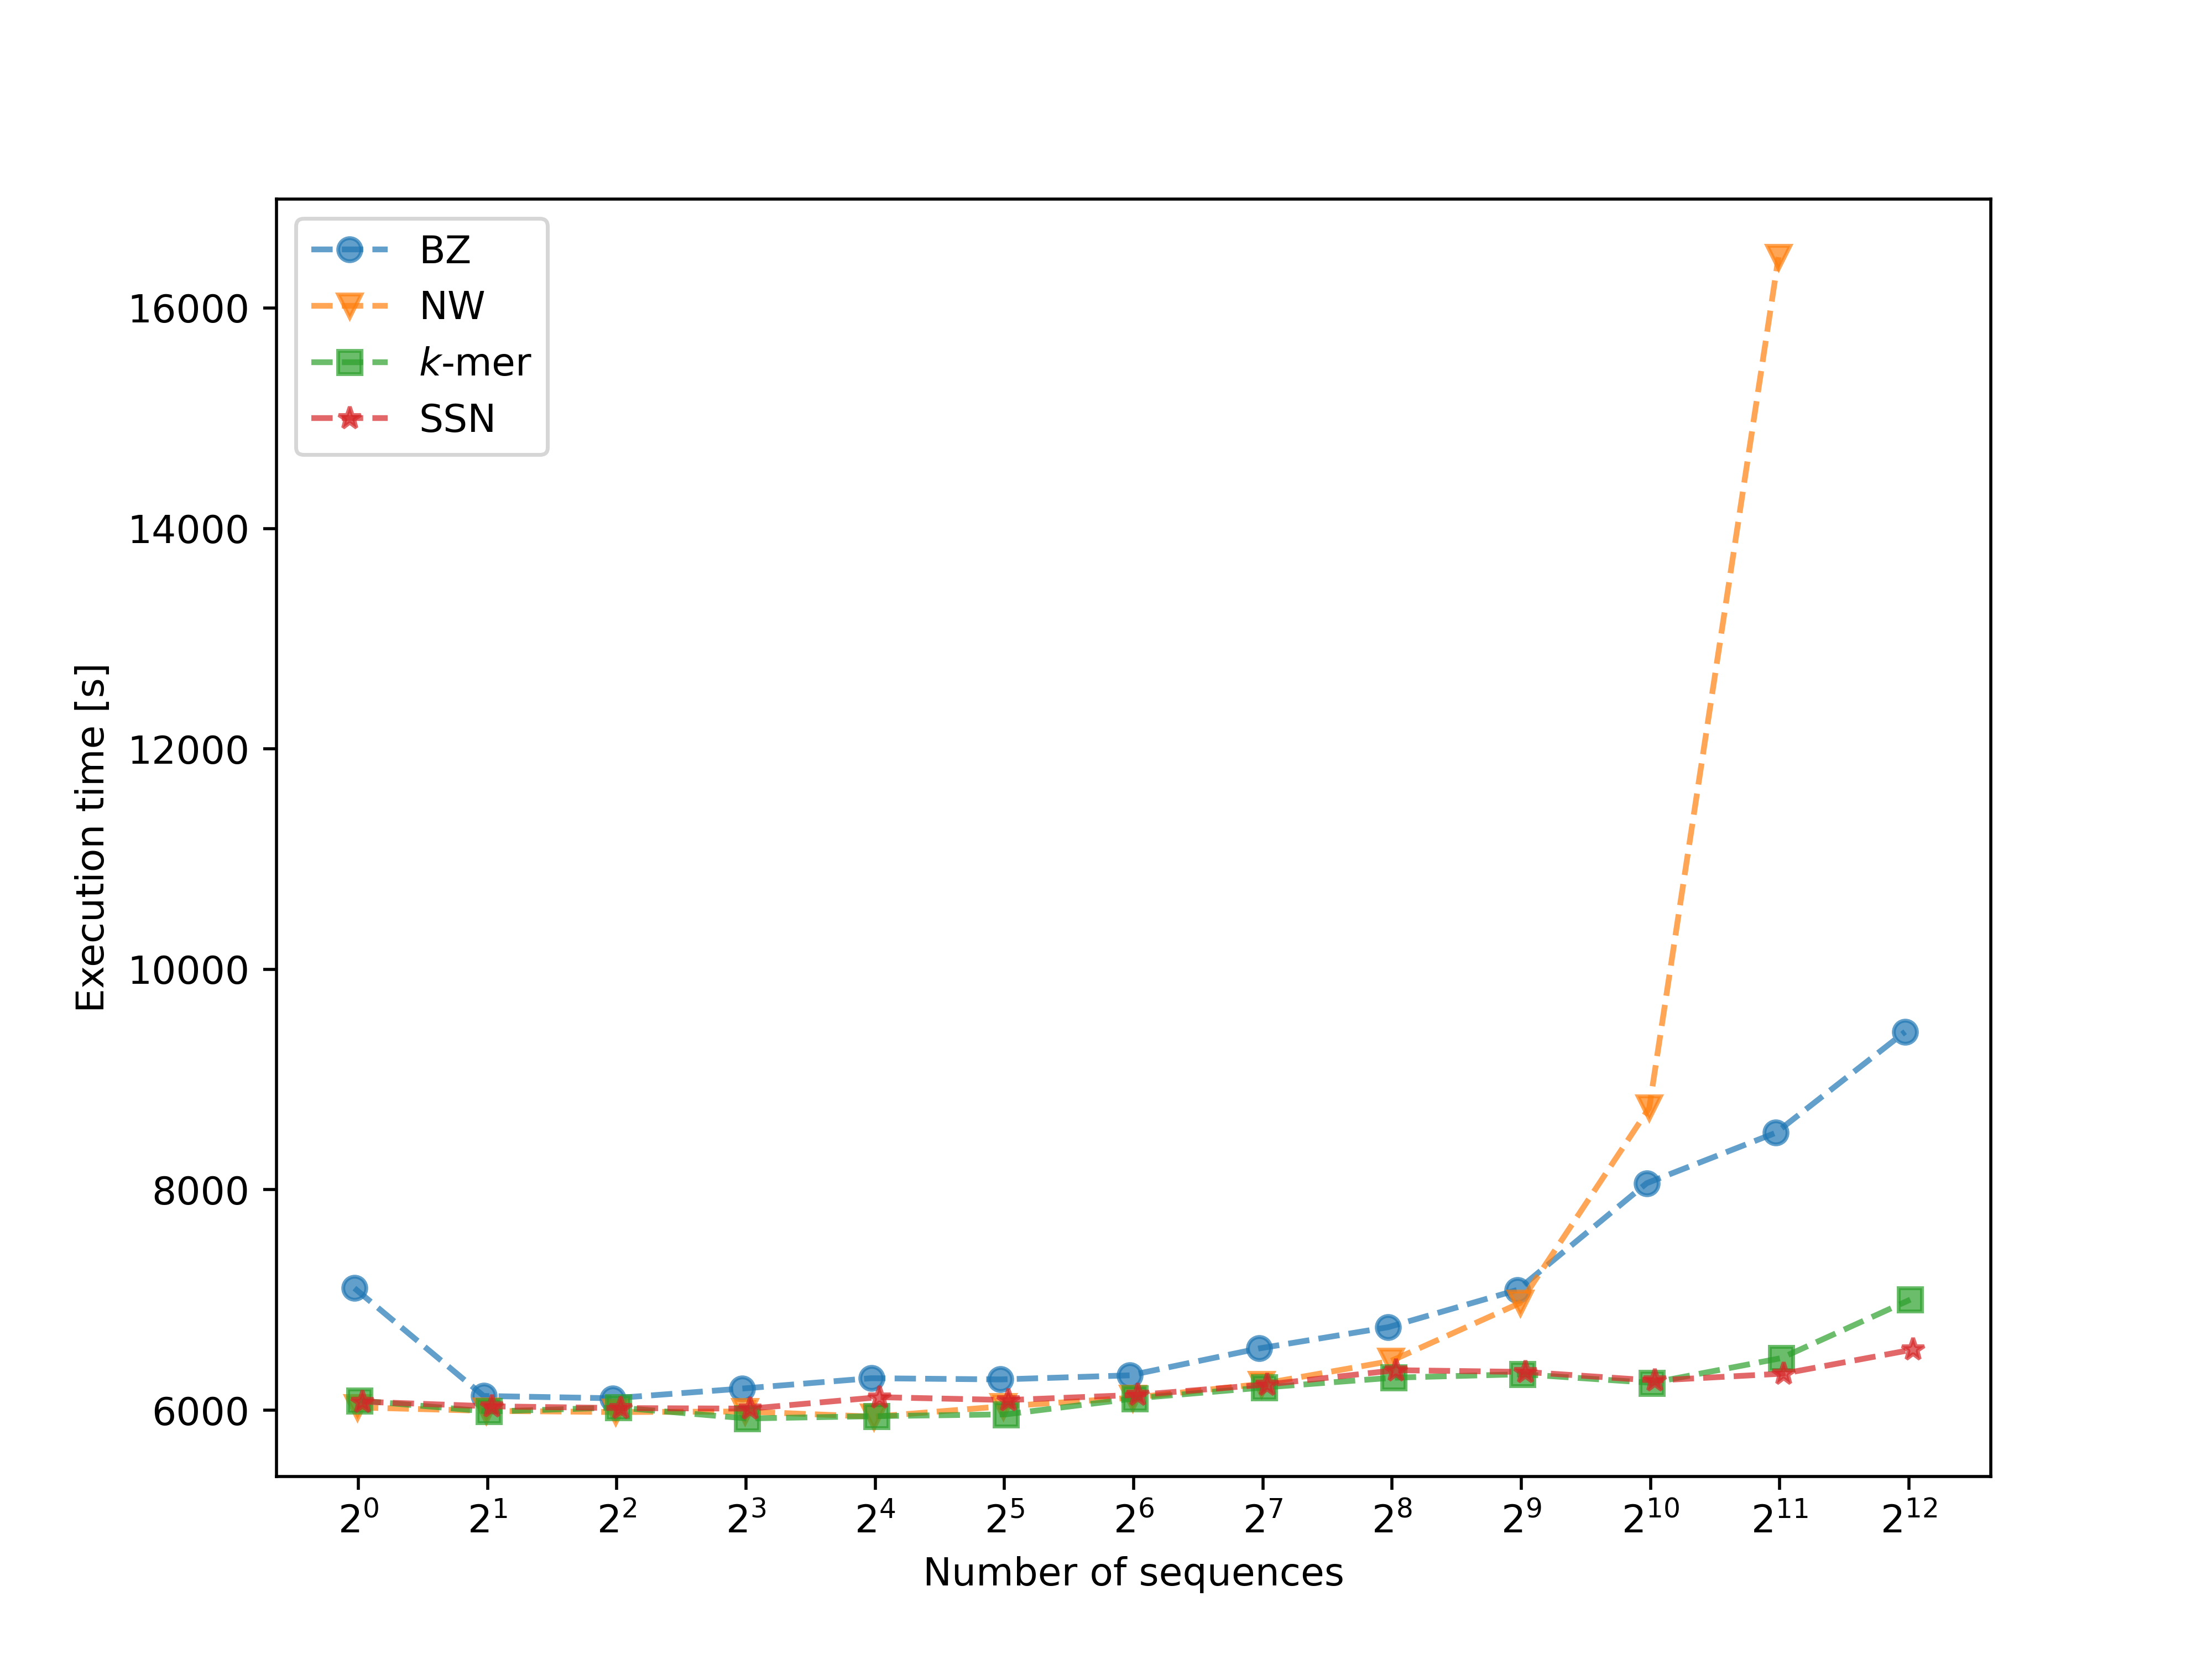
\includegraphics[width=\textwidth]{picture_experiment_duration.png}
                    \end{center}
                    \caption{
                        Metagenomic identification execution time.
                    }\label{Picture:Experiment:Duration}
                \end{figure}

                \begin{table}\centering
                    \caption{Metagenomic identification execution time.}\label{Table:Experiment:Duration}
                    \begin{tabular}{|c||c|c|c|c|}
                        \hline
                        \multirow{2}{*}{\textbf{Number of sequences}} & \multicolumn{4}{|c|}{\textbf{Execution time [s]}} \\
                                        & \textbf{NP} & \textbf{NW} & \textbf{$k$-mer} & \textbf{ANN} \\ \hline \hline
                                        1 & 7107 & \textbf{6025} & 6087 & 6077\\ \hline
                                        2 & 6129 & 5994 & \textbf{5988} & 6035\\ \hline
                                        4 & 6108 & \textbf{5983} & 6024 & 6019\\ \hline
                                        8 & 6196 & 5988 & \textbf{5925} & 6014\\ \hline
                                        16 & 6290 & \textbf{5941} & 5946 & 6118\\ \hline
                                        32 & 6279 & 6035 & \textbf{5962} & 6092\\ \hline
                                        64 & 6316 & 6113 & \textbf{6107} & 6139\\ \hline
                                        128 & 6560 & 6238 & \textbf{6206} & 6233\\ \hline
                                        256 & 6753 & 6446 & \textbf{6295} & 6363\\ \hline
                                        512 & 7091 & 6972 & \textbf{6326} & 6347\\ \hline
                                        1024 & 8059 & 8743 & \textbf{6248} & 6269\\ \hline
                                        2048 & 8517 & 16461 & 6472 & \textbf{6332}\\ \hline
                                        4096 & 9433 & \textbf{timeout} & 7003 & 6550\\ \hline

                    \end{tabular}
                \end{table}

                \paragraph{Conclusions}
                The method using the modified Needleman-Wunsch algorithm exhibited the fastest increase in execution time for metagenomic identification. The sharp rise is due to the time-consuming process of comparing sequences with each other. Despite reducing the number of sequences being classified, the execution time using this method exceeded that of metagenomic identification for all sequences.

                The methods using $k$-mer embeddings and ANN showed comparable execution times, with a slight advantage for the former. Both methods use sequence representations for comparison, resulting in a slower increase in the time needed to build the dissimilarity matrix. These methods performed faster than metagenomic identification for all sequences. In the case of the ANN, the shorter execution time for $4096$ sequences could be due to the simultaneous computation of embeddings for all sequences using the GPU.

            \subsubsection{Experiment 2: Metagenomic identification quality}
                \paragraph{Objective}
                Examining the quality of metagenomic identification using the implemented methods in comparison to the metagenomic identification of all sequences.

                \paragraph{Assumptions}
                \begin{enumerate}
                    \item {
                        Sequences clustering is deterministic.
                    }
                    \item {
                        \texttt{BLASTn} is deterministic and always returns the same results for a given sequence and specified parameters.
                    }
                    \item {
                        In the case where it is not possible to compute the quality for a given metagenomic identification run, a quality value of $0$ is assumed. This value is not considered when calculating the weighted average quality.
                    }
                  \end{enumerate}


        \subsection{Performance Measures}
            Quality of metagenomic identification was measured using a modified Jaccard index, expressed by equation~\ref{Equation:Quality}. The measure was used to compare the quality of metagenomic identification performed using the implemented methods against metagenomic identification without the use of a processing pipeline.

            \begin{equation}
                \text{Q} = \frac{
                    \sum_{r \in (O(R) \cap O(E))} R_{r}
                }{
                    \sum_{r \in (O(R) \cup O(E))} R_{r}
                }
                \label{Equation:Quality}
            \end{equation}

            where:
            \begin{align*}
                R &- \text{set of reference results,} \\
                E &- \text{set of obtained results,} \\
                R_{r} &- \text{number of results in reference set assigned to the organism $r$} \\
                O(X) &- \text{set of unique organisms, for which results were assigned in the set $X$}
            \end{align*}

            To compare the quality of multiple metagenomic identification runs, the weighted average quality, defined by equation~\ref{Equation:WeightedAverageQuality}, was used.
            
            \begin{equation}
                Q_{\text{avg}} = \sum_{c \in C} \frac{n_c}{n} Q_c
                \label{Equation:WeightedAverageQuality}
            \end{equation}

            where:
            \begin{align*}
            C &- \text{set of metagenomic identification runs,} \\
            Q_c &- \text{quality of metagenomic identificationn $c$,} \\
            n_c &- \text{number of input sequences for metagenomic identification $c$,}\\
            n   &- \text{number of input sequences $n = \sum_{c \in C} n_{c}.$}
            \end{align*}

                  

                \paragraph{Results}
                The quality of the classification was calculated using the measure expressed by equation~\ref{Equation:Quality} for the implemented methods in comparison to the full metagenomic identification. Figure~\ref{Picture:Experiment:Quality} shows a graph of classification quality as a function of the number of input sequences, with detailed quality results provided in Table~\ref{Table:Experiment:Quality}. The weighted average quality calculated using equation~\ref{Equation:WeightedAverageQuality} for the method with the modified Needleman-Wunsch algorithm was $0.899$, for the $k$-mer embedding method it was $0.921$, and for the method using the artificial neural network, it was $0.944$.

                \begin{figure}[!htb]
                    \begin{center}
                        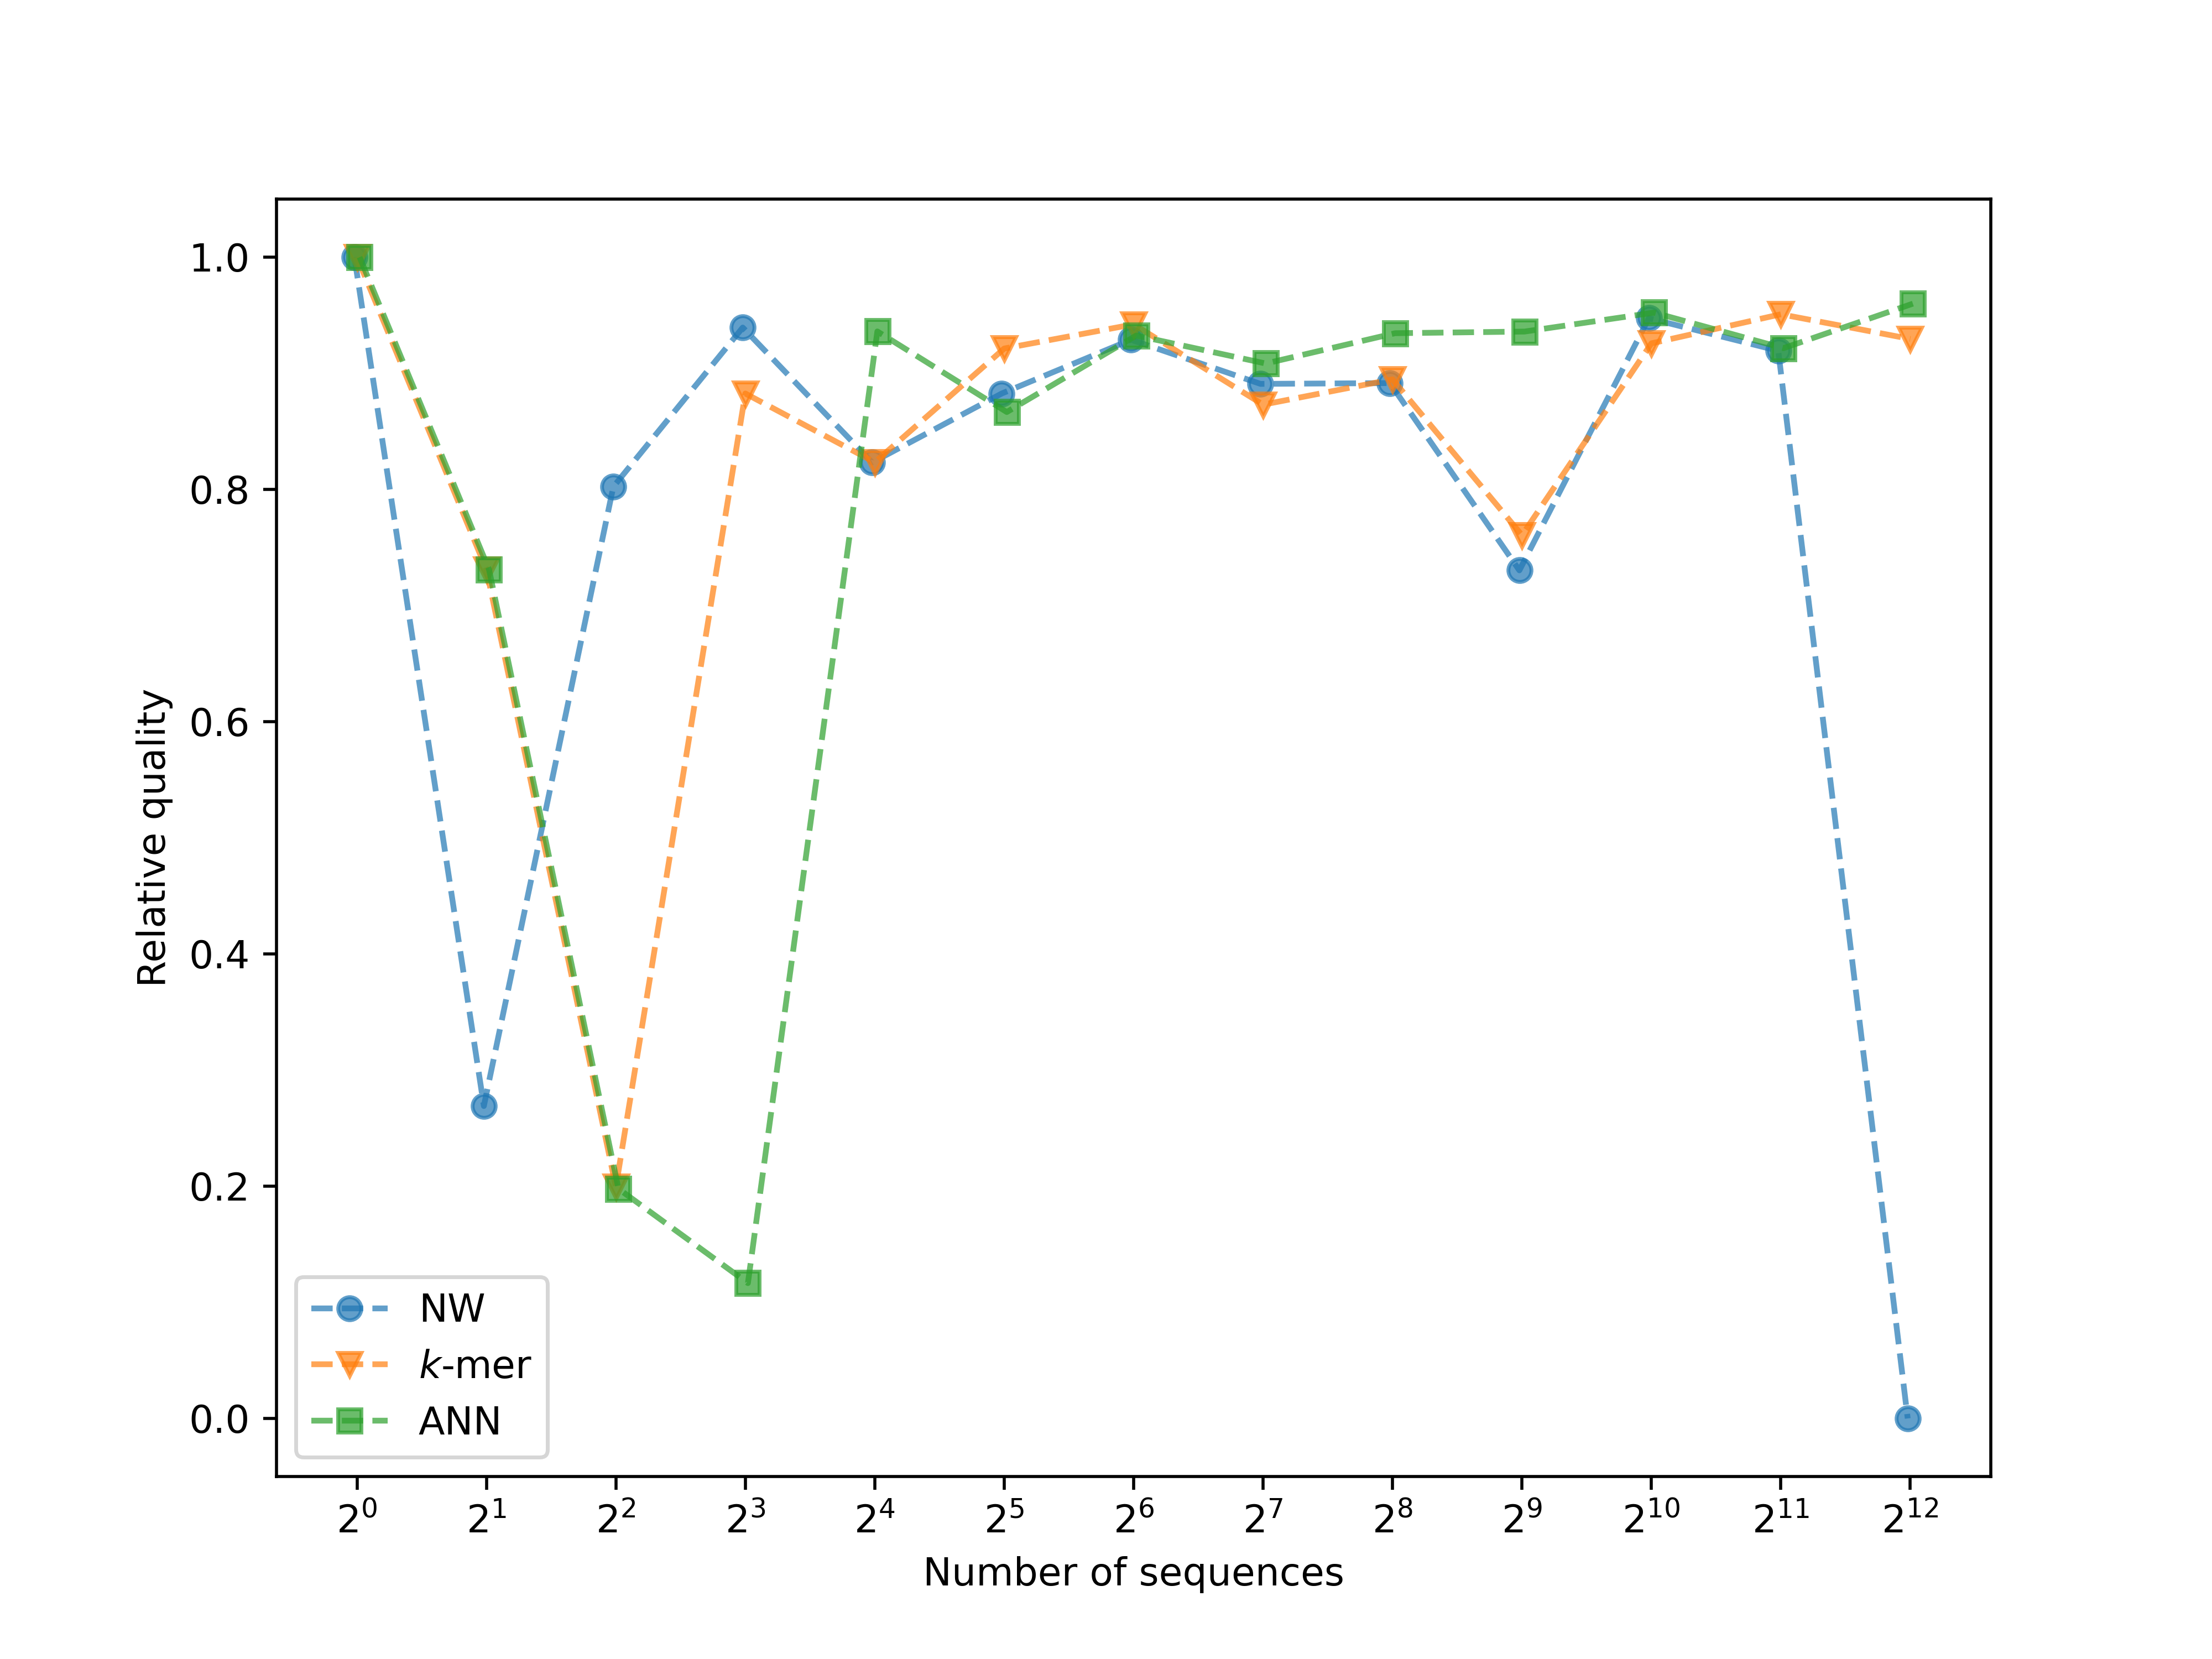
\includegraphics[width=\textwidth]{picture_experiment_quality.png}
                    \end{center}
                    \caption{
                        Metagenomic identification quality.
                    }\label{Picture:Experiment:Quality}
                \end{figure}

                \begin{table}\centering
                    \caption{Metagenomic identificationn quality.}\label{Table:Experiment:Quality}

                    \begin{tabular}{|c|c|c|c|}
                        \hline
                        \multirow{2}{*}{\textbf{Number of sequences}} & \multicolumn{3}{|c|}{\textbf{Method}} \\
                        & \textbf{NW} & \textbf{$k$-mer} & \textbf{ANN} \\ \hline \hline
                        1 & \textbf{1.0} & \textbf{1.0} & \textbf{1.0}\\ \hline
                        2 & 0.27 & \textbf{0.73} & \textbf{0.73}\\ \hline
                        4 & \textbf{0.8} & 0.2 & 0.2\\ \hline
                        8 & \textbf{0.94} & 0.88 & 0.12\\ \hline
                        16 & 0.82 & 0.82 & \textbf{0.94}\\ \hline
                        32 & 0.88 & \textbf{0.92} & 0.87\\ \hline
                        64 & 0.93 & \textbf{0.94} & 0.93\\ \hline
                        128 & 0.89 & 0.87 & \textbf{0.91}\\ \hline
                        256 & 0.89 & 0.89 & \textbf{0.93}\\ \hline
                        512 & 0.73 & 0.76 & \textbf{0.94}\\ \hline
                        1024 & \textbf{0.95} & 0.93 & \textbf{0.95}\\ \hline
                        2048 & 0.92 & \textbf{0.95} & 0.92\\ \hline
                        4096 & 0.0 & 0.93 & \textbf{0.96}\\ \hline
                    \end{tabular}
                \end{table}

                \paragraph{Conclusions}
                All implemented methods achieved very good classification quality results, exceeding $0.7$ in cases where the number of groups was significantly larger than the number of input sequences. The weighted average quality for all methods also reached a high value.

                The method using the artificial neural network achieved the best weighted average quality, slightly outperforming the $k$-mer embedding method and the method with the modified Needleman-Wunsch algorithm. The artificial neural network method owes its result to the model's consideration of the full sequence structure, which allowed for a better determination of dissimilarity between sequences.

    \section{Discussion}
        \subsection{Interpretation of Results}
            The results of the experiments partially confirmed the expectations set at the beginning of the research. All methods achieved satisfactory metagenomic identification quality. The method utilizing the artificial neural network performed particularly well, achieving the best weighted average classification quality while maintaining execution time comparable to the method based on $k$-mer embeddings. The low metagenomic identification quality with a small number of input sequences may be due to the inappropriate selection of group representatives, caused by too few available sequences. Therefore, the implemented methods should only be used in cases where the number of input sequences exceeds a certain threshold, and their use significantly reduces the time required for the metagenomic identification process. For the data tested, this condition is met for $128$ sequences, where the metagenomic identification quality was no less than $0.87$, and the use of any grouping method reduced the time by at least 5 minutes, resulting in a $5\%$ acceleration compared to the metagenomic identification of all sequences. The use of the artificial neural network allowed for an improvement in classification quality compared to other methods. In addition to achieving good classification quality, it does not lag behind classical methods.

        \subsection{Limitations}
            \subsubsection{Experiments Duration}
                The full process of metagenomic identification of DNA sequences for each method and each experimental subset took approximately 5 days, which led to the limitation of the number of experiments to single run and subset size to $4096$ sequences.

            \subsubsection{Single Dataset}  
                In work, only one sample from the chosen dataset was used. The selection of a sample containing DNA sequences from the human skin microbiome might have limited the space of analyzed sequences, which could have influenced the experimental results, as the both the artificial neural network and the experiments used DNA sequences from the same microbiome.

            \subsubsection{Single Dissimilarity Matrix}
                The use of a single dissimilarity matrix for all sequences limits the number of input sequences, as the matrix build time of matrix scales quadratically with the number of sequences.

        \subsection{Possible Improvements}
            \subsubsection{Architecture of Artificial Neural Network}
                The proposed artificial neural network architecture is not flexible and is only suitable for analyzing sequences of similar lengths. It would be possible to modify the model's architecture to incorporate recurrent neural networks (RNNs) and transformers, enabling the processing of sequences with varying lengths. RNNs and transformers could replace the first part of the model, which currently relies on convolutional layers. They would be used to create embeddings, which would later be processed by linear layers to generate an embedding that preserves dissimilarity properties.

            \subsubsection{Batching sequences}
                Creating a single dissimilarity matrix for very large samples is not optimal, as it significantly impacts the performance of the method. To address this issue, pre-clustering the sequences into batches can provide a solution. Processing in batches may reduce quality but allows for maintaining a short execution time.

            \subsubsection{Automatated Determination Of The Number of Groups}
                Current approach takes the number of created groups as a parameter, which can influence the quality of the results. For very similar sequences, a large number of groups is excessive and does not improve the results. Conversely, for highly diverse sequences, a low number of groups can reduce quality. Automating the determination of the optimal number of groups could solve the issue and minimize the need for fine-tuning 

    \section{Conclusions}
        \subsection{Summary of Findings}
            The experiments demonstrated that the method based on artificial neural networks outperforms traditional approaches in terms of quality, while maintaining execution times comparable to those of the classical $k$-mer method. This highlights the potential of neural networks for improving performance without significant computational overhead.

        \subsection{Future Research Directions}
        Future research could focus on utilizing artificial neural networks as an independent tool for metagenomic identification. Another promising direction is the application of artificial neural networks for dimensionality reduction of genetic sequences, which may improve efficiency and performance in various analyses.


\subsubsection*{Author contributions}

P.G and R.N. identified the problem, P.G. designed the approach, downloaded the data, implemented the software, performed numerical experiments, P.G. and R.N. prepared the draft. All authors have read and agreed to the published version of the manuscript.

\subsubsection*{Funding}

A statutory Research Grant from the Institute of Computer Science, Warsaw University of Technology, supports this work.



    %%=============================================================%%
    %% BACKMATTER
    %%=============================================================%%

    \backmatter

    %%=============================================================%%
    %% BIBLIOGRAPHY
    %%=============================================================%%

    \bibliography{bibliography}

\end{document}
